%Version 3.1 December 2024
% See section 11 of the User Manual for version history
%
%%%%%%%%%%%%%%%%%%%%%%%%%%%%%%%%%%%%%%%%%%%%%%%%%%%%%%%%%%%%%%%%%%%%%%
%%                                                                 %%
%% Please do not use \input{...} to include other tex files.       %%
%% Submit your LaTeX manuscript as one .tex document.              %%
%%                                                                 %%
%% All additional figures and files should be attached             %%
%% separately and not embedded in the \TeX\ document itself.       %%
%%                                                                 %%
%%%%%%%%%%%%%%%%%%%%%%%%%%%%%%%%%%%%%%%%%%%%%%%%%%%%%%%%%%%%%%%%%%%%%

%%\documentclass[referee,sn-basic]{sn-jnl}% referee option is meant for double line spacing

%%=======================================================%%
%% to print line numbers in the margin use lineno option %%
%%=======================================================%%

%%\documentclass[lineno,pdflatex,sn-basic]{sn-jnl}% Basic Springer Nature Reference Style/Chemistry Reference Style

%%=========================================================================================%%
%% the documentclass is set to pdflatex as default. You can delete it if not appropriate.  %%
%%=========================================================================================%%

%%\documentclass[sn-basic]{sn-jnl}% Basic Springer Nature Reference Style/Chemistry Reference Style

%%Note: the following reference styles support Namedate and Numbered referencing. By default the style follows the most common style. To switch between the options you can add or remove �Numbered� in the optional parenthesis. 
%%The option is available for: sn-basic.bst, sn-chicago.bst%  
 
%%\documentclass[pdflatex,sn-nature]{sn-jnl}% Style for submissions to Nature Portfolio journals
%%\documentclass[pdflatex,sn-basic]{sn-jnl}% Basic Springer Nature Reference Style/Chemistry Reference Style
\documentclass[pdflatex,sn-mathphys-num]{sn-jnl}% Math and Physical Sciences Numbered Reference Style
%%\documentclass[pdflatex,sn-mathphys-ay]{sn-jnl}% Math and Physical Sciences Author Year Reference Style
%%\documentclass[pdflatex,sn-aps]{sn-jnl}% American Physical Society (APS) Reference Style
%%\documentclass[pdflatex,sn-vancouver-num]{sn-jnl}% Vancouver Numbered Reference Style
%%\documentclass[pdflatex,sn-vancouver-ay]{sn-jnl}% Vancouver Author Year Reference Style
%%\documentclass[pdflatex,sn-apa]{sn-jnl}% APA Reference Style
%%\documentclass[pdflatex,sn-chicago]{sn-jnl}% Chicago-based Humanities Reference Style

%%%% Standard Packages
%%<additional latex packages if required can be included here>

\usepackage{graphicx}%
\usepackage{multirow}%
\usepackage{amsmath,amssymb,amsfonts}%
\usepackage{amsthm}%
\usepackage{mathrsfs}%
\usepackage[title]{appendix}%
\usepackage{xcolor}%
\usepackage{textcomp}%
\usepackage{manyfoot}%
\usepackage{booktabs}%
\usepackage{algorithm}%
\usepackage{algorithmicx}%
\usepackage{algpseudocode}%
\usepackage{listings}%
\usepackage{caption} % 추가
\usepackage{subcaption} % 추가
\usepackage{fontspec} %


% --- XeLaTeX용 폰트 설정
\usepackage{fontspec}
\usepackage[space]{xeCJK} % 한글용 추가
\setCJKmainfont{Noto Sans KR} % 마찬가지
%%%%

%%%%%=============================================================================%%%%
%%%%  Remarks: This template is provided to aid authors with the preparation
%%%%  of original research articles intended for submission to journals published 
%%%%  by Springer Nature. The guidance has been prepared in partnership with 
%%%%  production teams to conform to Springer Nature technical requirements. 
%%%%  Editorial and presentation requirements differ among journal portfolios and 
%%%%  research disciplines. You may find sections in this template are irrelevant 
%%%%  to your work and are empowered to omit any such section if allowed by the 
%%%%  journal you intend to submit to. The submission guidelines and policies 
%%%%  of the journal take precedence. A detailed User Manual is available in the 
%%%%  template package for technical guidance.
%%%%%=============================================================================%%%%

%% as per the requirement new theorem styles can be included as shown below
\theoremstyle{thmstyleone}%
\newtheorem{theorem}{Theorem}%  meant for continuous numbers
%%\newtheorem{theorem}{Theorem}[section]% meant for sectionwise numbers
%% optional argument [theorem] produces theorem numbering sequence instead of independent numbers for Proposition
\newtheorem{proposition}[theorem]{Proposition}% 
%%\newtheorem{proposition}{Proposition}% to get separate numbers for theorem and proposition etc.

\theoremstyle{thmstyletwo}%
\newtheorem{example}{Example}%
\newtheorem{remark}{Remark}%

\theoremstyle{thmstylethree}%
\newtheorem{definition}{Definition}%

\raggedbottom
%%\unnumbered% uncomment this for unnumbered level heads

\begin{document}

\title[Article Title]{A Scalable Approach for Large Molecular Systems: A Validation of Fragment molecular orbital-based Variational Quantum Eigensolver on the \(\mathrm{LiCoO_2}\)}
%Calculating Ground-State-Energy of \(\mathrm{LiCoO_2}\) by using Fragment molecular orbital-based Variational Quantum Eigensolver
% Benchmark

%%=============================================================%%
%% GivenName	-> \fnm{Joergen W.}
%% Particle	-> \spfx{van der} -> surname prefix
%% FamilyName	-> \sur{Ploeg}
%% Suffix	-> \sfx{IV}
%% \author*[1,2]{\fnm{Joergen W.} \spfx{van der} \sur{Ploeg} 
%%  \sfx{IV}}\email{iauthor@gmail.com}
%%=============================================================%%

\author[1]{\fnm{Choe} \sur{Yoonho}}\email{cyh195535@hanyang.ac.kr}

\author[1]{\fnm{Kim} \sur{Doyeon}}\email{rlaehdus3333@hanyang.ac.kr}


\author[1]{\fnm{Kim} \sur{Doha}}\email{lichkim01@hanyang.ac.kr}

\author*[1,2]{\fnm{Kwon} \sur{Younghun}}\email{yyhkwon@hanyang.ac.kr}


\affil[1]{\orgdiv{Department of applied Phisics}, \orgname{Hanyang University}, \orgaddress{\city{Ansan}, \postcode{15588}, \state{Republic of Korea}}}

\affil[2]{\orgdiv{Department of Intelligence, Information, and Quantum}, \orgname{Hanyang University}, \orgaddress{\city{Ansan}, \postcode{15588}, \state{Republic of Korea}}}


%%==================================%%
%% Sample for unstructured abstract %%
%%==================================%%

\abstract{The Variational Quantum Eigensolver (VQE) is a quantum algorithm for estimating ground-state energies, with promising applications in material science, drug discovery, and battery research. A key challenge is the limited number of qubits available on current quantum devices, which restricts the size of molecular systems that can be studied. To address this limitation, we apply the Fragment Molecular Orbital (FMO) method in combination with VQE, referred to as FMO-VQE. This approach divides a system into smaller fragments, making the quantum calculations more tractable. While earlier studies demonstrated this method only for hydrogen clusters, we extend the application to lithium cobalt oxide, a widely used cathode material in lithium-ion batteries. Using FMO-VQE, we estimate the ground-state energy of this complex system while reducing the number of required qubits from 24 to 14, without significant loss of accuracy compared to classical methods. This reduction highlights the potential of FMO-VQE to overcome hardware limitations and make quantum simulations of larger molecules feasible. The results suggest a practical path for applying near-term quantum computers to real-world challenges, opening opportunities for advancements in battery Industry and pharmaceutical design.}

%%================================%%
%% Sample for structured abstract %%
%%================================%%

% \abstract{\textbf{Purpose:} The abstract serves both as a general introduction to the topic and as a brief, non-technical summary of the main results and their implications. The abstract must not include subheadings (unless expressly permitted in the journal's Instructions to Authors), equations or citations. As a guide the abstract should not exceed 200 words. Most journals do not set a hard limit however authors are advised to check the author instructions for the journal they are submitting to.
% 
% \textbf{Methods:} The abstract serves both as a general introduction to the topic and as a brief, non-technical summary of the main results and their implications. The abstract must not include subheadings (unless expressly permitted in the journal's Instructions to Authors), equations or citations. As a guide the abstract should not exceed 200 words. Most journals do not set a hard limit however authors are advised to check the author instructions for the journal they are submitting to.
% 
% \textbf{Results:} The abstract serves both as a general introduction to the topic and as a brief, non-technical summary of the main results and their implications. The abstract must not include subheadings (unless expressly permitted in the journal's Instructions to Authors), equations or citations. As a guide the abstract should not exceed 200 words. Most journals do not set a hard limit however authors are advised to check the author instructions for the journal they are submitting to.
% 
% \textbf{Conclusion:} The abstract serves both as a general introduction to the topic and as a brief, non-technical summary of the main results and their implications. The abstract must not include subheadings (unless expressly permitted in the journal's Instructions to Authors), equations or citations. As a guide the abstract should not exceed 200 words. Most journals do not set a hard limit however authors are advised to check the author instructions for the journal they are submitting to.}

\keywords{VQE, Quantum Computing, Lithium-ion batteries}


%%\pacs[JEL Classification]{D8, H51}

%%\pacs[MSC Classification]{35A01, 65L10, 65L12, 65L20, 65L70}

\maketitle

\section{Introduction}\label{sec1}
\cite{RN50,RN48,RN47}
The ground-state energy of a molecule is fundamental to understanding molecular bonds and their structural properties. 
This information is essential across a wide range of chemical research areas, including the development of new drugs materials\cite{RN66,RN69}, and advanced cathode materials for secondary batteries \cite{RN117,RN118,RN75}. 
Currently, classical computers are used to calculate the ground-state energy of molecules.
However, as the number of atoms in a molecule increases, or as the atomic number of the elements involved grows, the complexity of the system also increases exponentially.
This results in a rapid rise in the number of particles and their interactions, which are represented in the molecule’s Hamiltonian. 
The need to process these interactions requires significant computational resources and memory. 
Consequently, calculating the ground-state energy of large molecules becomes increasingly challenging on classical computers.

Quantum computers, which are an emerging technology, offer a promising alternative. Unlike classical computers, quantum computers use qubits, having superpositions of  0 and 1 states. 
This allows quantum computers to potentially calculate the ground-state energy of a molecule much more efficiently. 
While classical computers require exponential increases in memory as the system size grows, quantum computers only need a polynomial increase in qubits to handle the same task. 
This enables quantum computers to process large molecules that would be infeasible for classical computers.
One approach to calculating the ground-state energy of a molecule on a quantum computer is the Quantum Phase Estimation (QPE) algorithm, which determines the eigenvalues and eigenstates of a unitary matrix [12-16]. 
However, QPE is highly accurate but requires a large number of qubits, which makes it impractical for current quantum devices, particularly noisy intermediate-scale quantum (NISQ) devices [17]. 
These devices are limited by noise, lack of precision, and a relatively small number of qubits, making it difficult to implement QPE effectively.

The Variational Quantum Eigensolver (VQE) is another algorithm designed to solve eigenvalue problems on NISQ-level quantum computers by combining both quantum and classical computing [18-21].
VQE uses a variational approach with constructing a parameterized trial wavefunction as a Quantum Circuit, 
which is iteratively adjusted until it converges to provide an upper bound for the ground-state energy. 
The quantum computer performs the expectation value calculations, while the classical computer optimizes the parameters of trial wavefunction.
Unlike QPE, VQE requires fewer qubits and allows for the optimization process to be handled by a classical computer, 
making it a promising candidate for commercial quantum computing applications in the NISQ era. 
Despite its potential, current quantum computers still face significant challenges, including errors and decreased accuracy as circuit depth increases. 
Additionally, the limited number of available qubits restricts the ability to calculate the ground-state energy of very large molecules. 
To address these issues, one promising approach is the Fragment Molecular Orbital-based Variational Quantum Eigensolver (FMO-VQE).
Initially proposed by Lim et al. [1], the FMO-VQE method applies the classical FMO technique, which divides a molecule into smaller fragments and calculates the ground-state energy for individual monomers and dimers [22-25]. 
These results are then used to estimate the total ground-state energy of the entire molecule. 
While Lim et al. demonstrated the FMO-VQE method on hydrogen clusters, its application to more complex molecules remain unexplored. 
This raises the question of whether the FMO-VQE approach is effective for real-world applications. 
In this study, we investigate the performance of FMO-VQE by considering \(\mathrm{LiCoO_2}\), a key material used as a cathode in lithium-ion batteries. We calculate the ground-state energy of \(\mathrm{LiCoO_2}\) and compare the results with those from classical computations, demonstrating the potential of FMO-VQE for handling complex materials like \(\mathrm{LiCoO_2}\).

\section{Methods}\label{sec2}

\subsection{Lithium-ion battery}\label{subsec2.1}
Lithium-ion batteries are widely used secondary batteries in various industries. A lithium-ion battery consists of a cathode material, an anode material, and an electrolyte, with lithium oxide typically used as the cathode material. This compound has a layered structure of CoO₂⁻, with \(\mathrm{Li^+}\) ions bonded between each layer. The energy charge of the battery depends on the extent to which the lithium ions are oxidized in the oxide [1-3].
Lithium is known to have limited reserves in the world, prompting the need for sustainable solutions [4]. One such solution is to maximize the energy charged per lithium ion. 
This is critical both in terms of conserving lithium resources and for advancing battery miniaturization[5, 6]. 
To calculate the amount of energy stored per lithium ion, it is essential to compute the ground state of the molecule. However, this calculation is typically done using classical methods, 
and the ability to calculate larger molecules or more complex combinations is limited.
In this study, we demonstrate the application of the VQE algorithm to \(\mathrm{LiCoO_2}\) molecules and highlight the potential of quantum computers in the field of battery development.
\begin{figure}[H]
  \centering
  \begin{subfigure}[b]{0.45\textwidth}
    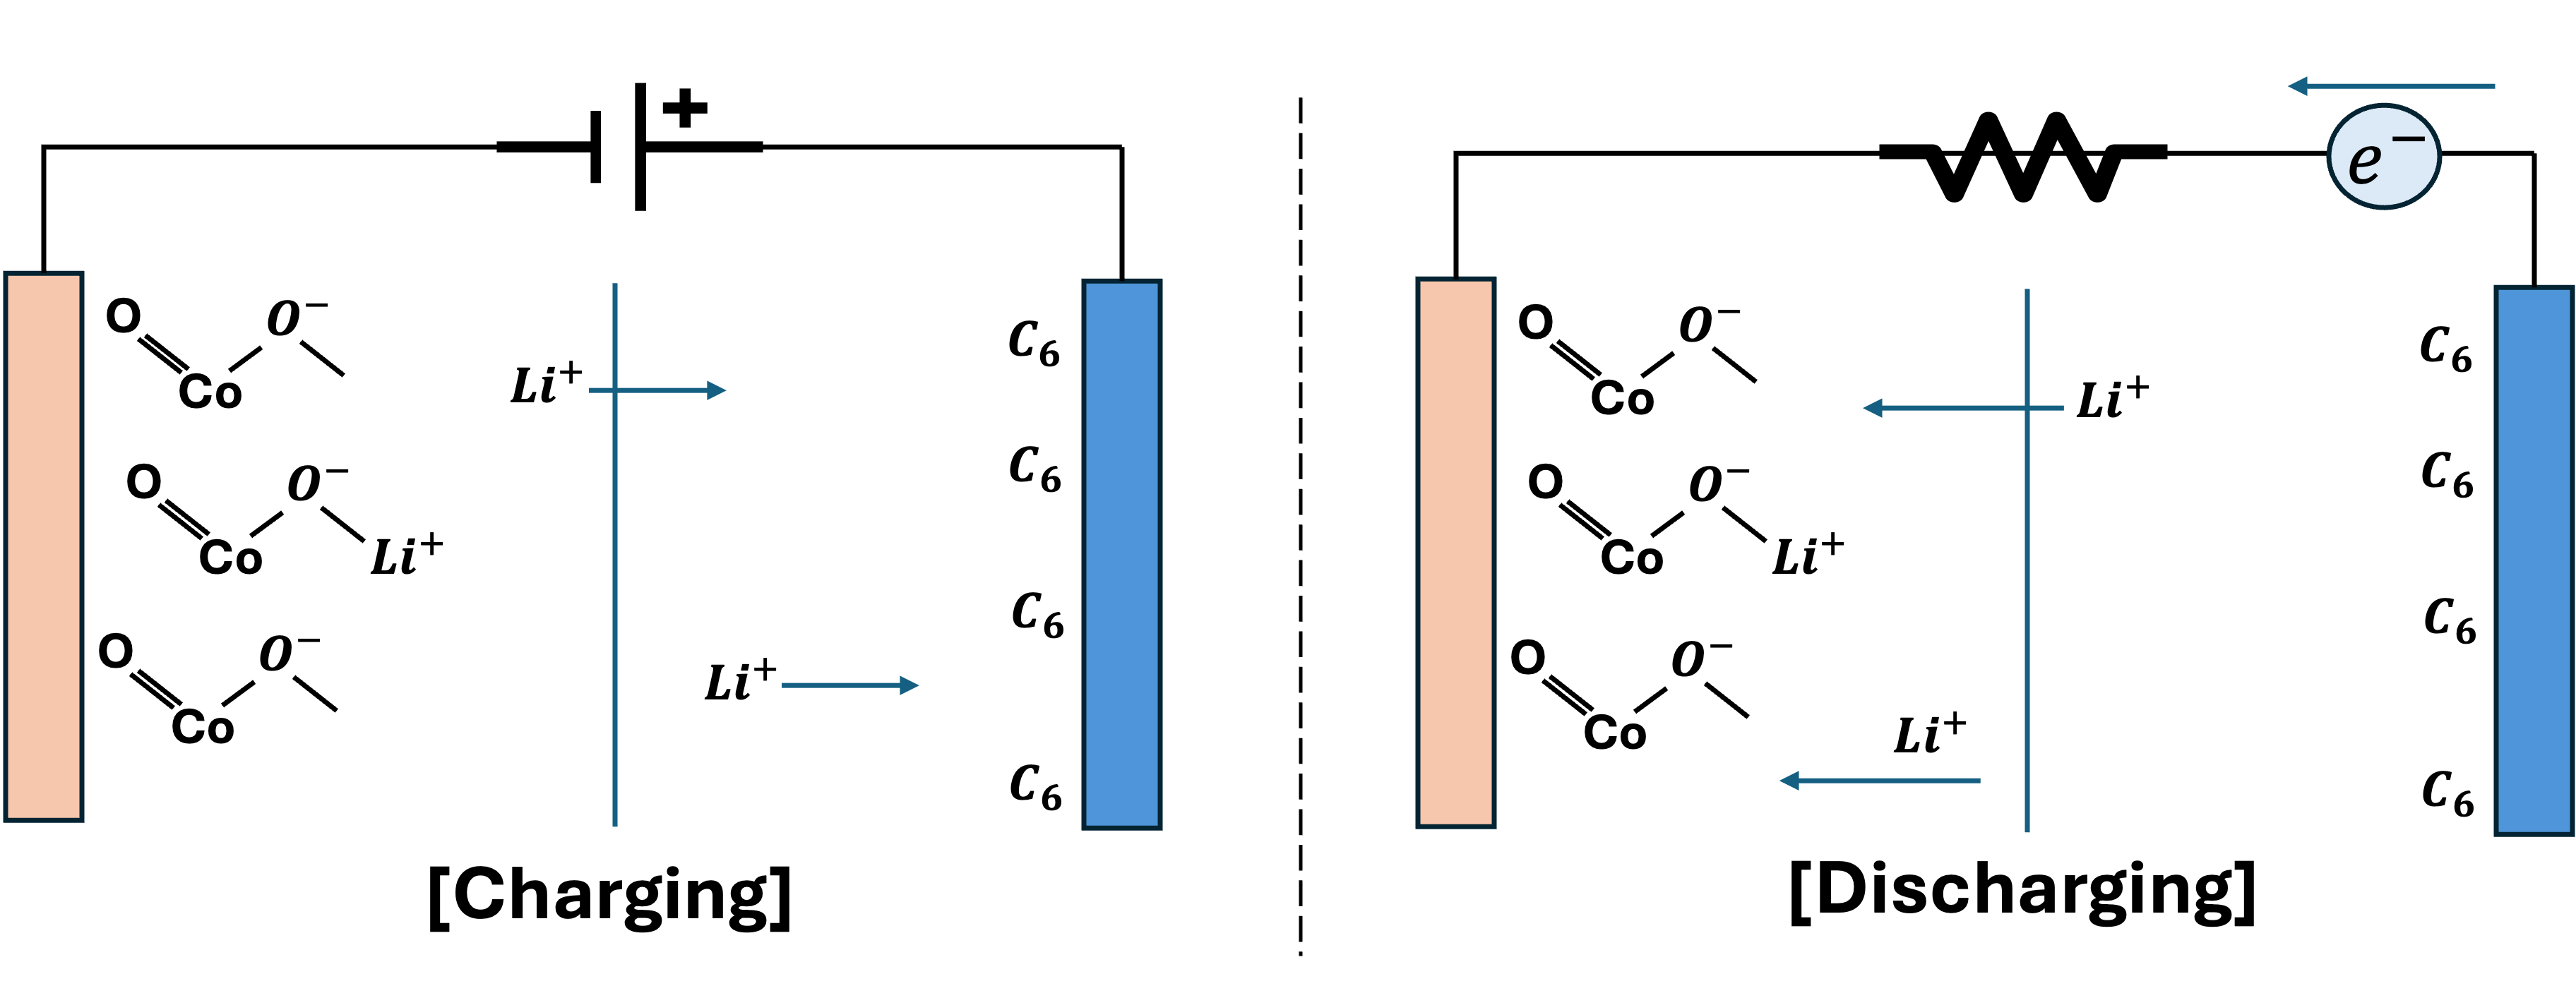
\includegraphics[width=\textwidth]{fig/Cha_discha.png}
    \caption{}
    \label{fig:first}
  \end{subfigure}
  \hfill
  %\vrule width 1pt  % 수직선 추가 (굵기: 1pt)
  \hfill
  \begin{subfigure}[b]{0.45\textwidth}
    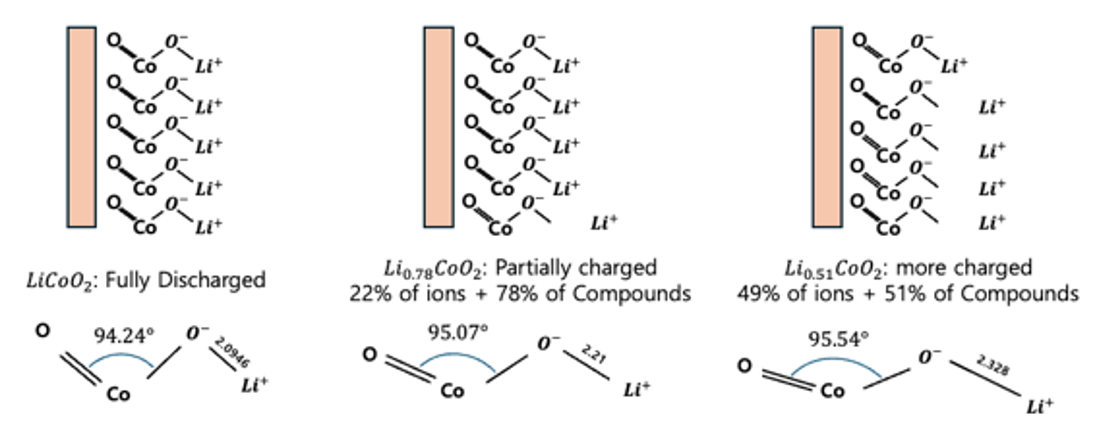
\includegraphics[width=\textwidth]{fig/char.png}
    \caption{}
    \label{fig:second}
  \end{subfigure}
  \caption{(a) a Schematic of battery charging and discharging. The red-colored elements represent the cathode, while the blue-colored elements represent the anode. The arrows represent the movement of lithium ions and electrons. (b) Depending on the oxidation state (denoted as x in \(\mathrm{Li_xCoO_2}\)) of each compound, the upper figure represents the relative number of lithium ions separated from the cathode, while the lower figure illustrates the average geometry of \(\mathrm{LiCoO_2}\).}
  \label{fig:two_figures_side_by_side}
\end{figure}
When a voltage is applied to the anode and cathode to supply electrons (i.e., during charging), the  \(\mathrm{Li^+}\) ions migrate to the anode. 
Upon discharging from this charged state, the \(\mathrm{Li^+}\) ions from the anode recombine with the cathode, as shown in the Fig. 1 (a) right, and current flows through the resistor. 
During this process, depending on the oxidation state of lithium, the average geometry of the molecular structure changes, as illustrated in Fig. 1 (b).
Therefore, the energy stored in the bulk can be estimated using this geometry. 
The energy of the molecule is calculated by assuming a gas-phase model, which treats the average oxide structure as a single molecule.

\subsection{VQE(Variational Quantum Eigensolver)}\label{subsec2.2}
\begin{figure}[htbp]
\centering
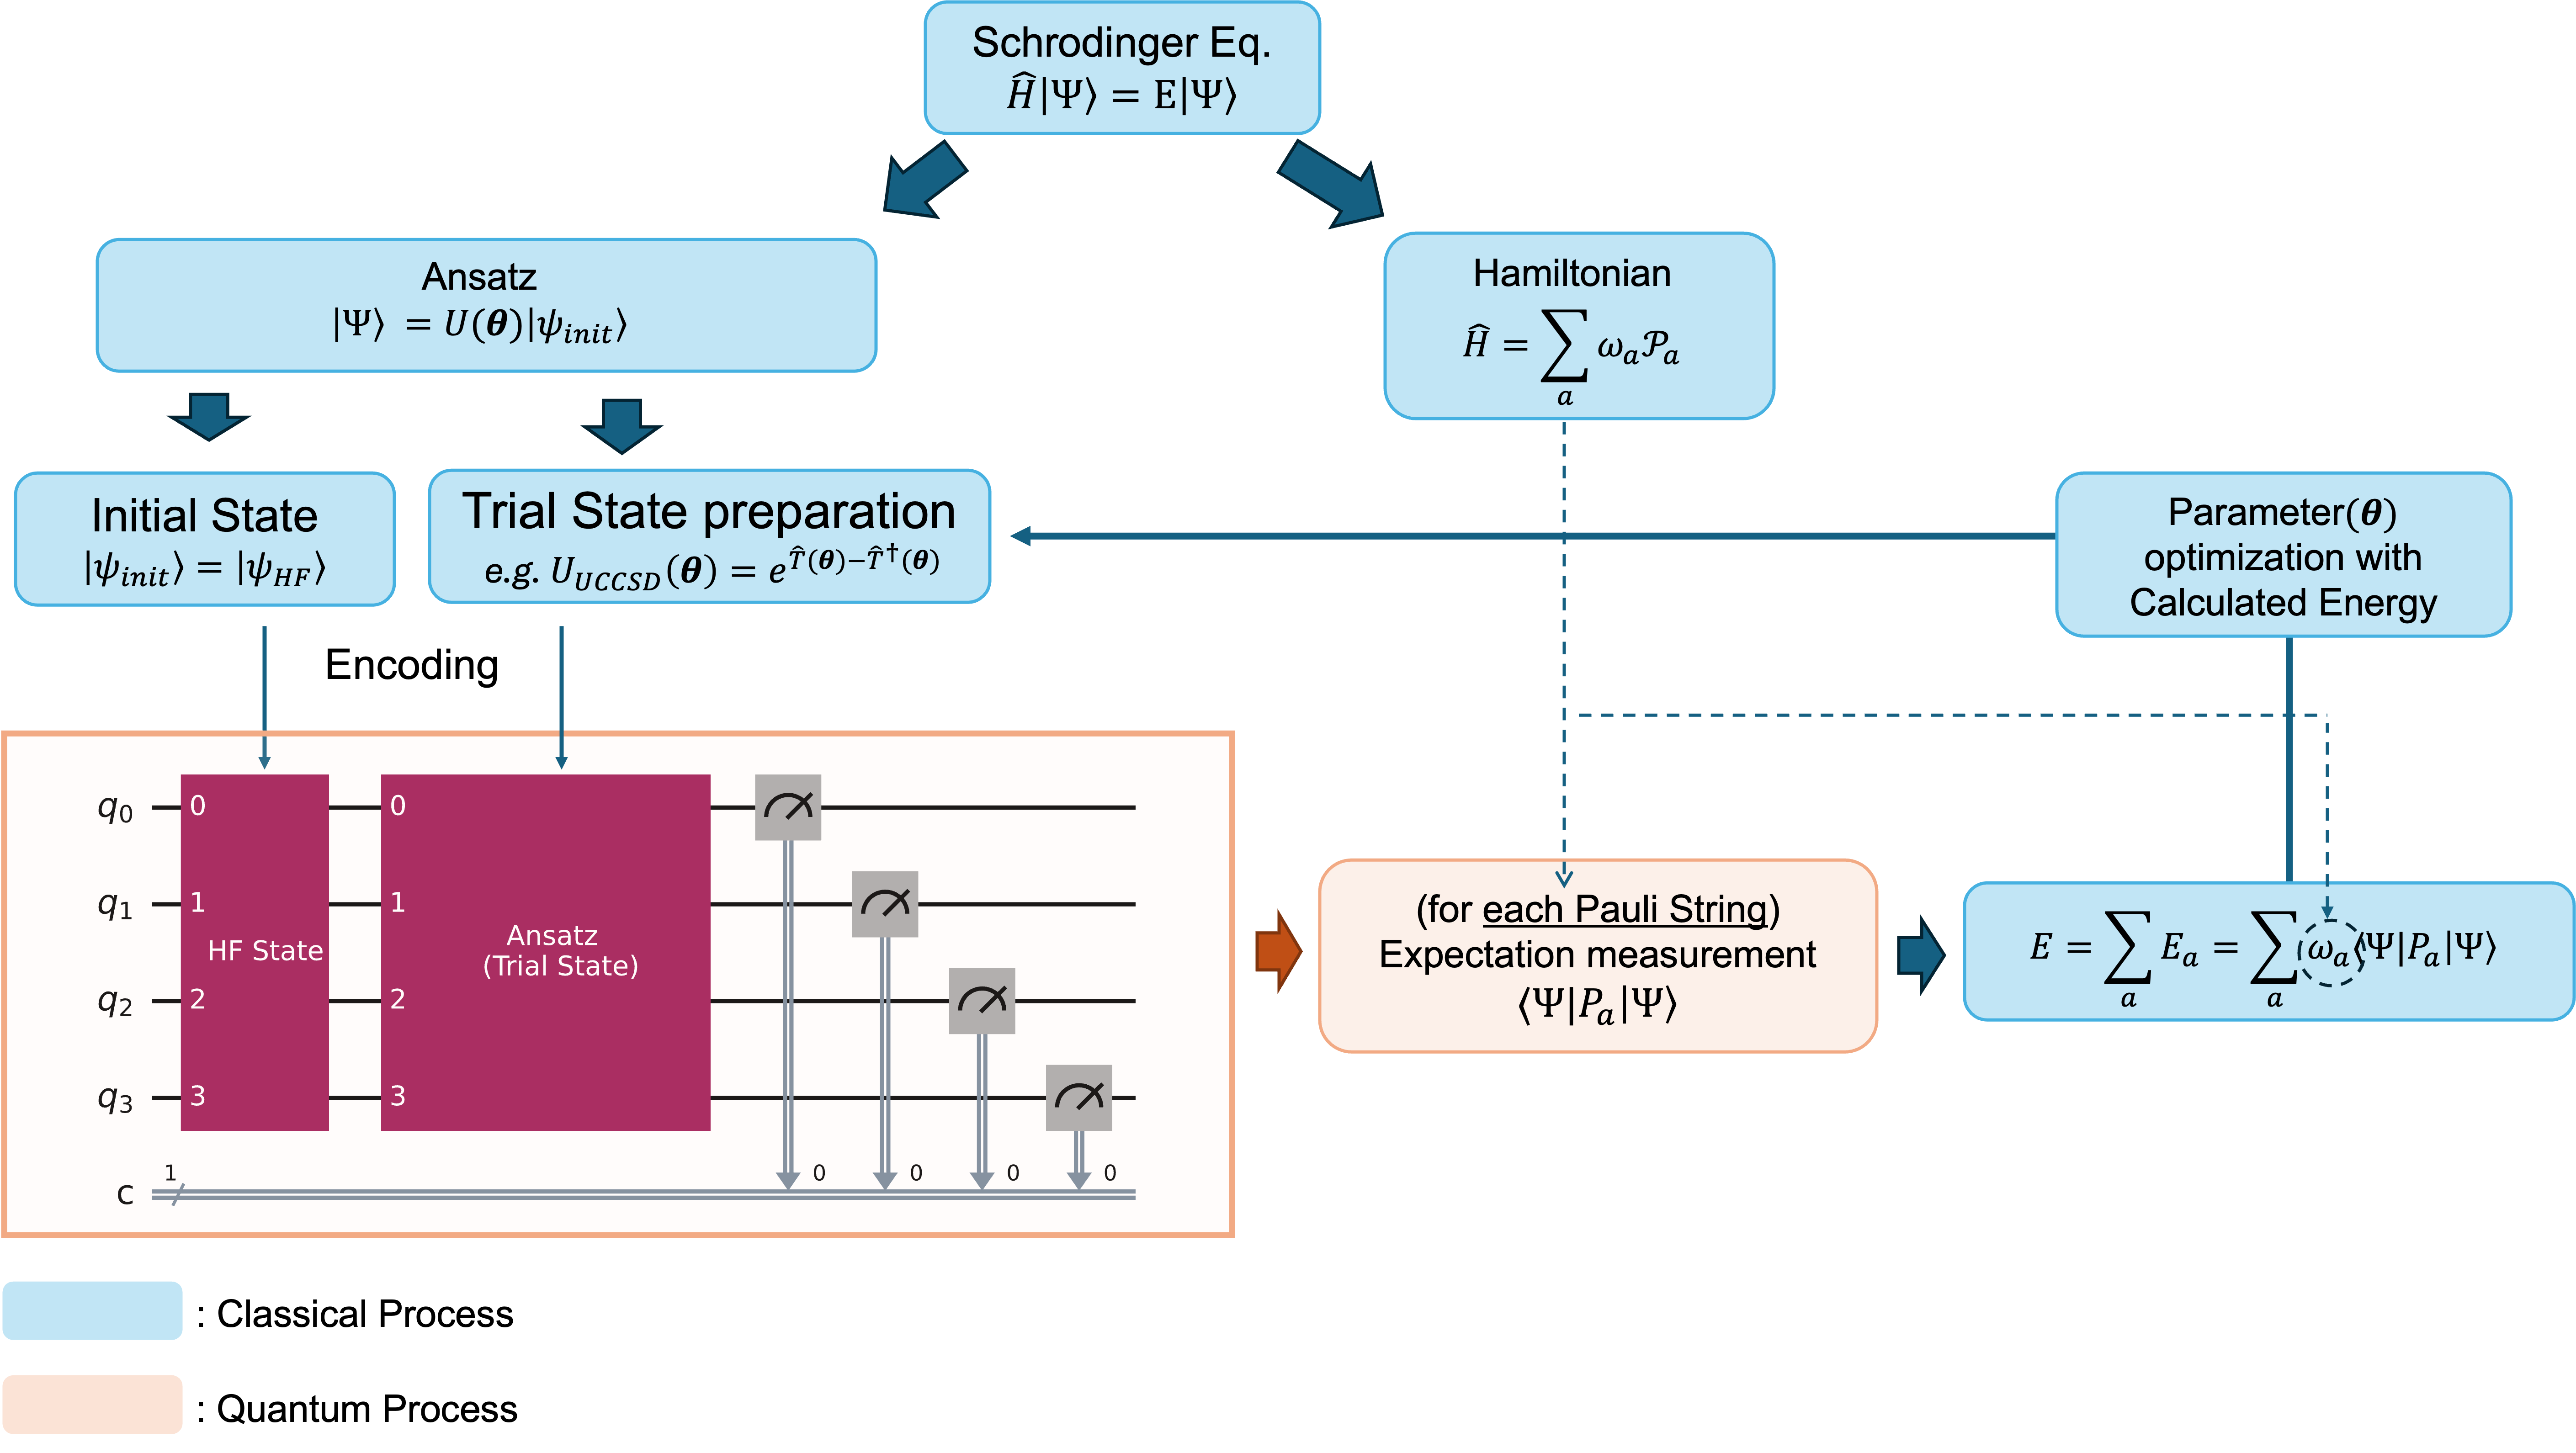
\includegraphics[width=0.8\textwidth]{fig/VQE_pipeline.png}
\caption{VQE Pipeline. Starting from the Schrödinger equation of the system, the process involves finding an appropriate measurement basis using the Hamiltonian, constructing an Ansatz to represent an arbitrary state with a parameterized quantum circuit, and finding the ground state energy through the variational method by performing measurements and updating the parameters}\label{Fig.2}
\end{figure}
The Variational Quantum Eigensolver (VQE) algorithm is an eigenvalue problem-solving method first proposed by Peruzzo et al [18]. 
It works by computing the energy in Hilbert space, providing an upper bound on the ground state energy according to the variational principle. 
VQE calculates the ground state energy of a system by measuring the energy on a quantum computer and performing optimization on a classical computer. 
To measure the energy of a system on a quantum computer, the Hamiltonian must be mapped to a form that can be represented as a quantum circuit. 
Additionally, an arbitrary quantum state needs to be encoded into the circuit for the measurement process.

\subsubsection{Hamiltonian}\label{subsec2.2.1}
The Hamiltonian of a molecule is represented by the Electronic Structure Hamiltonian as follows:
\begin{align}
\hat{H}_{el} 
&= \sum_{i} \frac{\nabla_{\mathbf{r}_i}^2}{m_i}
+ \sum_{I} \sum_{i} \frac{Z_I e^2}{\left| \mathbf{R}_I - \mathbf{r}_i \right|}
+ \sum_{i} \sum_{j>i} \frac{e^2}{\left| \mathbf{r}_i - \mathbf{r}_j \right|}
\end{align}
where \(r_i\) denotes the position vector of the i-th electron, 
\(R_I\) denotes the position of the I-th nucleus, and \(Z_I\) is the atomic number of the I-th nucleus. 
To map this Hamiltonian to the Pauli gates, we express it in second quantized form using fermionic creation/annihilation operators [7-9], as follows:
\begin{align}
\hat{H} 
&= \sum_{p,q} h_{pq} \, \hat{a}_p^{\dagger} \hat{a}_q
+ \frac{1}{2} \sum_{p,q,r,s} h_{pqrs} \, \hat{a}_p^{\dagger} \hat{a}_q^{\dagger} \hat{a}_r \hat{a}_s
\end{align}
\begin{equation*}
\text{where,} \quad 
h_{pq} = \langle \phi_p \vert \hat{H}_{\mathrm{el}} \vert \phi_q \rangle, \quad
h_{pqrs} = \langle \phi_p \, \phi_q \vert \hat{H}_{\mathrm{el}} \vert \phi_r \, \phi_s \rangle
\end{equation*}
Fermionic operators can be mapped to Pauli gates through widely adopted mapping methods such as Jordan-Wigner mapping, Parity mapping, and bravyi-kitaev mapping [10, 11]. 
In this experiment, we will use the Parity mapping method. 
Parity mapping expresses the creation/annihilation operator through a Pauli gate by corresponding the parity of the i-th qubit to the parity of the electron occupancy of the i-th orbital. 
In this case, the parity of the \(\alpha-\) spin and \(\beta-\) spin of the molecule can be utilized to reduce the number of qubits required by two. 
The resulting Hamiltonian of the mapping is represented by a Pauli string \(P_a\) and its weights or linear coefficients \(\omega_a\) as shown below.
\begin{equation}
\hat{H} = \sum_{a} \omega_{a} \, \mathcal{P}_{a}
\end{equation}

\subsubsection{Ansatz}\label{subsec2.2.2}
To apply the variational principle, a parameterized quantum state is required, and in VQE, this is represented by a parameterized quantum circuit, 
referred to as an Ansatz. In general, the Ansatz can be constructed using either hardware-efficient methods or Hamiltonian-inspired approaches.
The performance of the ansatz is difficult to evaluate, and it is not known a priori which ansatz is better for different systems. 
In this experiment, we compare two representative types of Ansatz, one hardware-efficient and the other Hamiltonian-inspired, and adopt the one yielding better results for our calculations.

\paragraph{TwoLocal(Efficient SU2) Ansatz} \leavevmode \newline
Since the quantum state of a single qubit can be represented on the Bloch sphere with two rotation gate, we take this idea as a basis. 
By treating the rotation gate angles as variational parameters and introducing entanglement—a defining property of multi-qubit systems—through CNOT gates, 
the quantum state of an arbitrary multi-qubit system can then be efficiently expressed in terms of these parameters.

\begin{figure}[htbp]
\centering
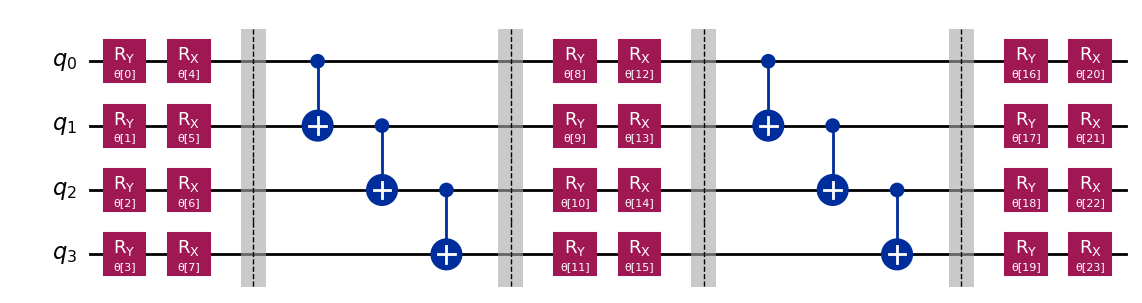
\includegraphics[width=0.8\textwidth]{fig/twolocal.png}
\caption{An example of a TwoLocal Ansatz for a 4-Qubit system with 2 repetitions. The regions represented by dashed lines and the gray area distinguish the layers. The regions represent-ed by Rx and Ry gates, which include the parameter θ, represent the "rotation layer", while the regions represented by CNOT gates correspond to the "entanglement layer".}\label{Fig.3}
\end{figure}
The construction of the TwoLocal Ansatz does not require an interpretation of the Hamiltonian. It is a representation of an arbitrary quantum state that is encoded in hardware, making it hardware-efficient.

\paragraph{UCCSD(Unitary Coupled Cluster Singles and Doubles) Ansatz} \leavevmode \newline
Through second quantization, we express the Hamiltonian operator in terms of the basis of the molecular orbitals of the system. Ultimately, 
the state we are looking for is represented in the same Hilbert space as the Hamiltonian. By using the same spin-orbitals as the basis, 
we can express any quantum state in the Hilbert space where the Hamiltonian exists. 

When the spin-orbital wavefunctions of a molecule are used as the basis, the quantum state can be represented in the CCSD form—incorporating only singles and doubles—within the Coupled-Cluster framework [12,13]. Furthermore, to encode this representation on a quantum circuit, it can be recast as a unitary operator, yielding the UCCSD (Unitary Coupled-Cluster Singles and Doubles) ansatz as shown below [14].

\begin{equation}
\vert \Phi(\mathbf{\theta})\rangle_{UCCSD} = e^{T-T^{\dagger}}\vert \Phi_{HF} \rangle
\end{equation}

\begin{equation}
\hat{T} = \hat{T}_1 + \hat{T}_2 \quad \text{(Cluster operator)}
\end{equation}

\begin{equation*}
\text{where,} \quad 
\hat{T}_1 = \sum_{i,a} c_i^a \, \hat{a}_a^{\dagger} \hat{a}_i, \quad
\hat{T}_2 = \sum_{i,j,a,b} t_{ij}^{ab} \, \hat{a}_a^{\dagger} \hat{a}_b^{\dagger} \hat{a}_j \hat{a}_i
\end{equation*}
Here, $\lvert \Phi_{HF} \rangle$ denotes the Hartree–Fock state. The states are represented by creation and annihilation operators, which can be encoded in quantum circuits using either Jordan-Wigner mapping or parity mapping. 

\subsubsection{Energy calculation}\label{subsec2.2.3}

The energy of the system for each interaction is evaluated by measuring the expectation value of each Pauli string in the Hamiltonian within the quantum circuits. 
\begin{equation}
E(\mathbf{\theta}) = \sum_{a} \omega_a \langle \Psi(\mathbf{\theta}) \vert \mathcal{P}_a \vert \Psi(\mathbf{\theta}) \rangle
\end{equation}

By iteratively performing these measurements and optimizing the ansatz parameters to minimize the energy,
an upper bound on the ground-state energy is obtained. 
\begin{equation}
E_{ground}\leq E_{VQE} = \min_{\mathbf{\theta}} E(\mathbf{\theta})
\end{equation}
The converged  value achieved corresponds to the ground-state energy estimated by the VQE algorithm for the system.

%The energy of the system is calculated by measuring the expectation value for each Pauli string in the Hamiltonian within these quantum circuits.
%By iterating over these measurements and optimizing the parameters of the ansatz to minimize the calculated energy, 
%an upper bound on the ground state energy is determined. 
%The resulting minimum corresponds to the ground state energy calculated by the VQE algorithm for the system.


\subsection{FMO (Fragmental Molecular orbital)}\label{subsec2.3}
\begin{figure}[H]
\centering
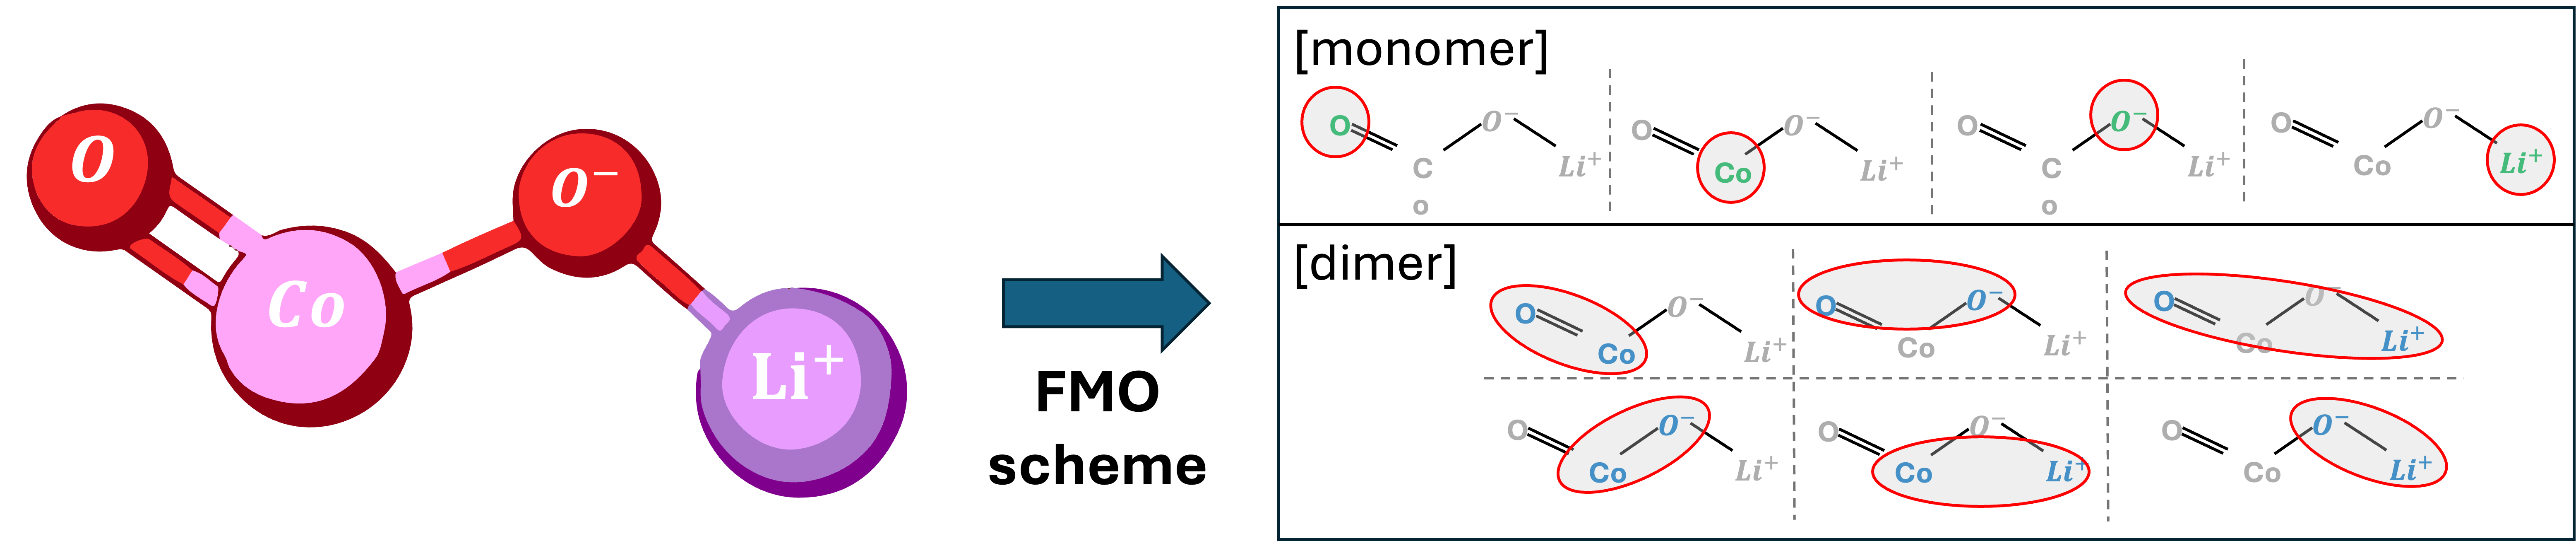
\includegraphics[width=0.8\textwidth]{fig/LiCoO2_FMO.png}
\caption{An example of the FMO scheme in \(\mathrm{LiCoO_2}\)}\label{Fig.4}
\end{figure}
The FMO method is a method that divides a whole molecular system into smaller system fragments and approximates the energy of the whole system by using the energy of one fragment (monomer) and the energy of pairs of fragments (dimers). When calculating the ground state energy of a molecule by the usual method, the computational complexity is exponential in the size of the system. However, the FMO method can effectively reduce the computational complexity by dividing a large system into parts. 
The FMO method has two main steps. The first is the FMO-based restricted Hartree-Fock (FMO-RHF) process, which calculates the RHF through the Hamiltonian of monomers and dimers. The Hamiltonian of monomer \(\mathrm{(\hat{H}_{A})}\) and the Hamiltonian of dimer\(\mathrm{(\hat{H}_{AB})}\) are as follows. 
\begin{equation}
\hat{H}_A = 
\sum_{i \in A} \Bigg[
    -\frac{\nabla_{\mathbf{r}_i}^2}{m_e}
    - \sum_I \frac{Z_I}{|\mathbf{r}_i - \mathbf{R}_I|}
    + \sum_{C \neq A}^{N_{\mathrm{tot}}} 
      \int d\mathbf{r}' \, \frac{\rho_J(\mathbf{r}')}{|\mathbf{r}_i - \mathbf{r}'|}
\Bigg]
+ \sum_{i<j \in A} \frac{1}{|\mathbf{r}_i - \mathbf{r}_j|}\label{eq5}
\end{equation}
\begin{equation}
\hat{H}_{AB} = 
\sum_{i \in A,B} \Bigg[
    -\frac{\nabla_{\mathbf{r}_i}^2}{m_e}
    - \sum_I \frac{Z_I}{|\mathbf{r}_i - \mathbf{R}_I|}
    + \sum_{C \neq A,B}^{N_{\mathrm{tot}}} 
      \int d\mathbf{r}' \, \frac{\rho_J(\mathbf{r}')}{|\mathbf{r}_i - \mathbf{r}'|}
\Bigg] + \sum_{i<j \in A,B} \frac{1}{|\mathbf{r}_i - \mathbf{r}_j|}
\end{equation}
(Where A,B are the respective fragments. C refers to the fragments that are not included in monomer A or dimer AB, and the term \(\rho_J(r')\) is the electric charge density of the fragments outside the monomer or dimer.) By calculating the RHF of each monomer and dimer through the Hamiltonian above, we can get \({E^\mathrm{FMO-RHF}}\), which can be expressed as follows.
\begin{equation}
E^{\mathrm{FMO2\!-\!RHF}} = E^{\mathrm{FMO1\!-\!RHF}} + \Delta E^{\mathrm{FMO2\!-\!RHF}}
\end{equation}
\begin{equation}
E^{\mathrm{FMO1\!-\!RHF}} = \sum_{A}^{N} E_A
\end{equation}
\begin{equation}
\Delta E^{\mathrm{FMO2\!-\!RHF}} = \sum_{A > B}^{N} \Big[ E_{IJ} - E_I - E_J \Big]
\end{equation}
In the above equations, N refers to all fragments. From the above equations, we can get the HF energy including the electrostatic potential of the whole molecule. The next step is to proceed with FMO based coupled-cluster (FMO-CC). This process is performed to obtain a more accurate value of the FMO-RHF energy, and since this process does not include the electrostatic potential, the Hamiltonian can be calculated using the Electronic Structure Hamiltonian defined earlier. The process of calculating the total energy \(E^\mathrm{FMO-CC}\) and correlation energy \(E^\mathrm{FMO-corr}\) obtained through FMO-CC is as follows.
\begin{equation}
E^{\mathrm{FMO}n\!-\!\mathrm{CC}} = E^{\mathrm{FMO}n\!-\!\mathrm{RHF}} + E^{\mathrm{FMO}n\!-\!\mathrm{corr}}
\end{equation}
\begin{equation}
E^{\mathrm{FMO2\!-\!corr}} = E^{\mathrm{FMO1\!-\!corr}} + \Delta E^{\mathrm{FMO2\!-\!corr}}
\end{equation}
\begin{equation}
E^{\mathrm{FMO1\!-\!corr}} = \sum_{A}^{N} E_A^{\mathrm{corr}}
\end{equation}
\begin{equation}
\Delta E^{\mathrm{FMO2\!-\!corr}} = \sum_{A>B}^{N} 
\left( E_{IJ}^{\mathrm{corr}} - E_I^{\mathrm{corr}} - E_J^{\mathrm{corr}} \right)
\end{equation}
In the above, the FMO-RHF and FMO-CC processes should be separated because the Hamiltonian used in the two processes may be different, and the FMO-CC process should proceed after the SCF calculation of FMO-RHF converges. However, in this experiment, the electrostatic potential term in the FMO-RHF Hamiltonian was approximated by ignoring it, so each process was carried out consecutively and the total energy was calculated from the obtained monomer and dimer energies as follows.

\subsection{FMO-VQE (Fragment molecular orbital-based Varational Quantum Eigensolver)}\label{subsec2.4}
\begin{figure}[H]
\centering
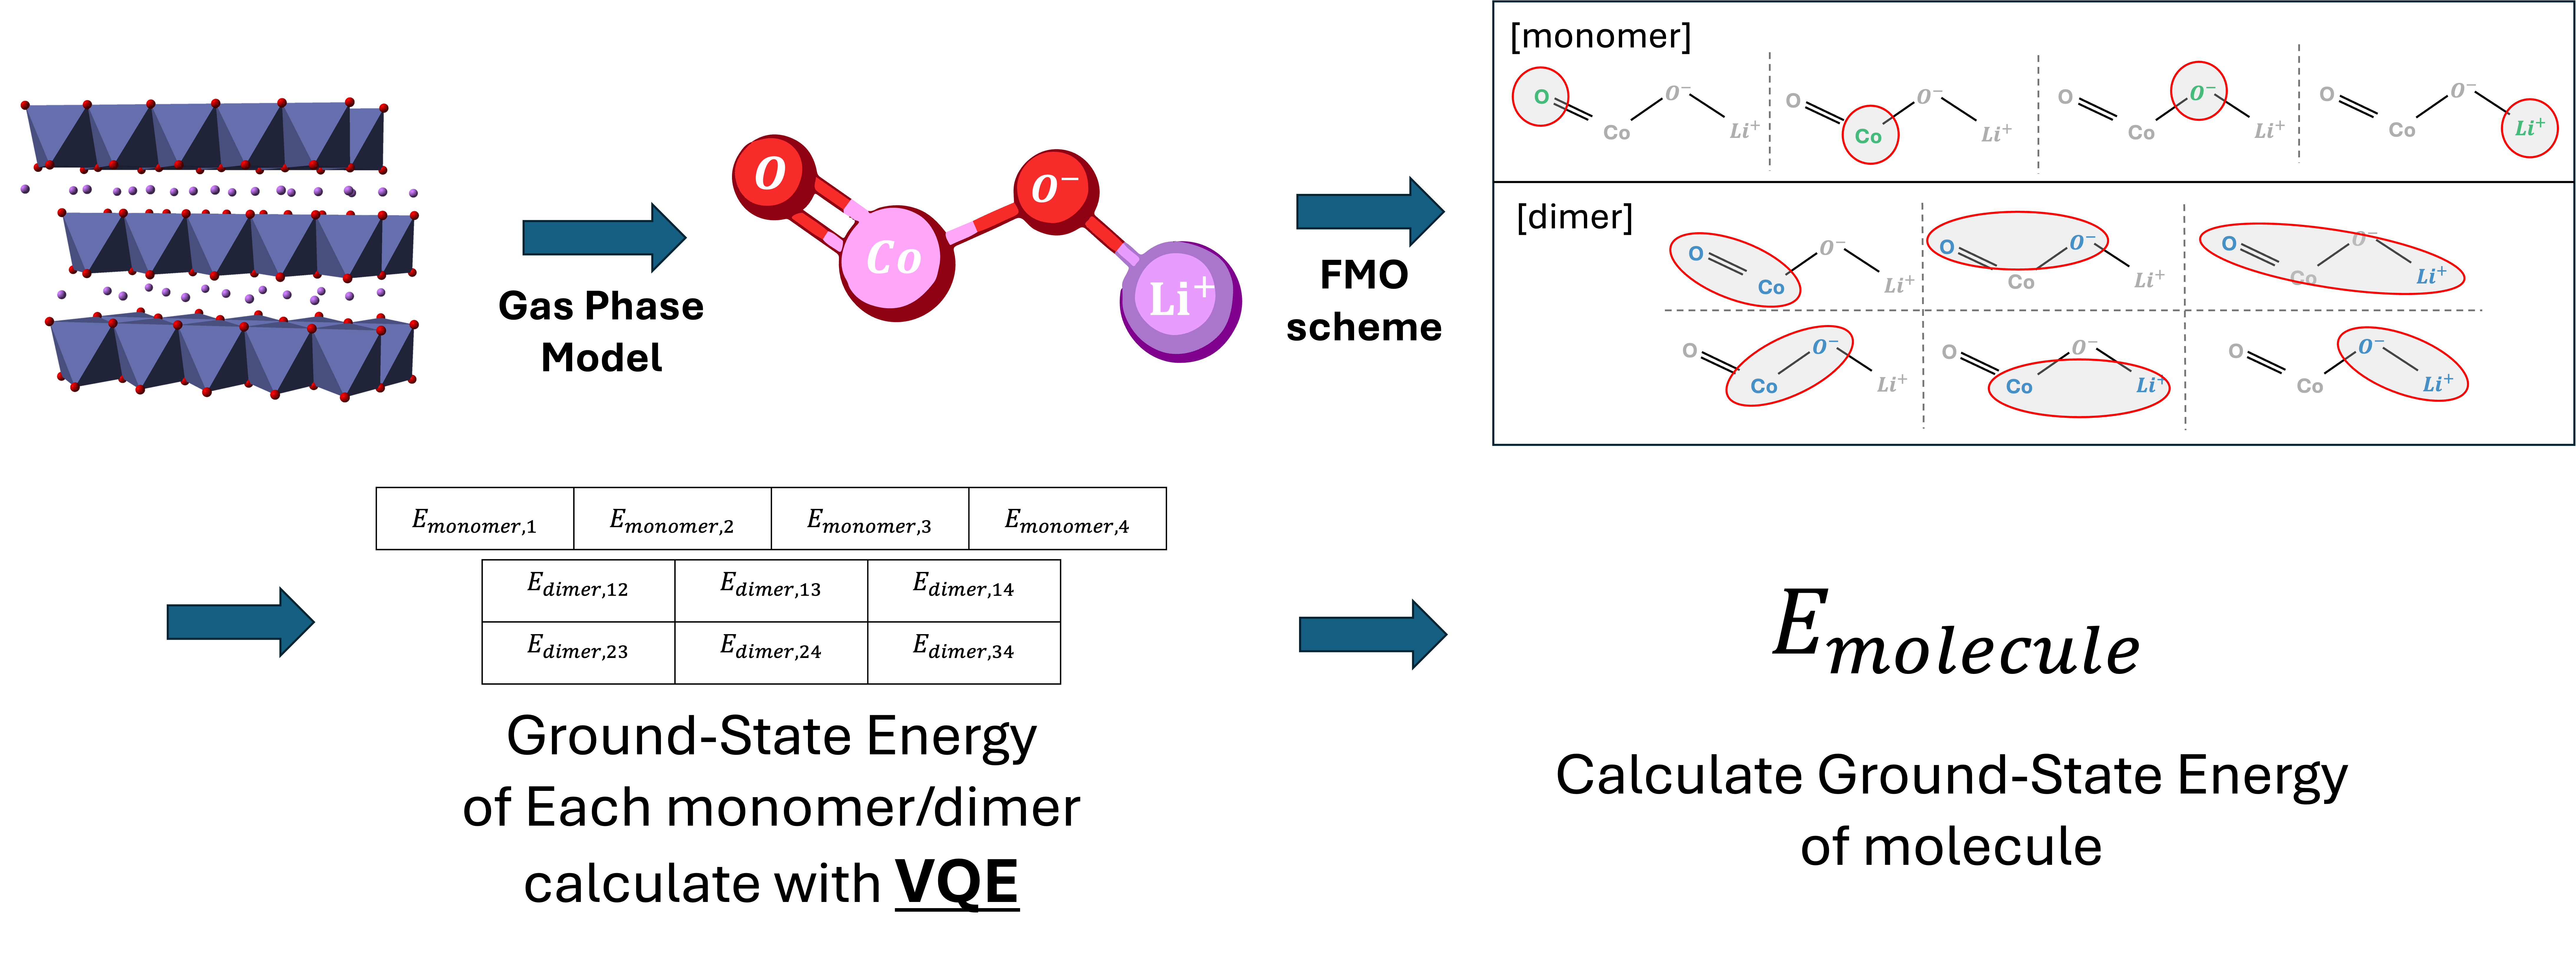
\includegraphics[width=0.8\textwidth]{fig/FMO_VQE_schme.png}
\caption{An illustration of applying the FMO/VQE method. 1) \(\mathrm{LiCoO_2}\) compound in the cathode material forms a layered structure, However, assuming a gas-phase model, it is considered that a single compound exists as a molecule. 2) The FMO scheme is applied to form monomers and dimers. 3) The ground state energy of each fragment is calculated using VQE. 4) The ground state energy of the entire molecule is then calculated using the energies of each fragment.}\label{Fig.5}
\end{figure}
FMO-VQE is an algorithm first introduced by Lim et al. that combines the VQE algorithm with the FMO method. In the VQE algorithm, the Hamiltonian is represented based on the molecular spin-orbitals, so it requires as many qubits as the number of molecular spin-orbitals. However, the number of qubits is currently limited, so the number of molecules that can be simulated in the existing VQE algorithm is limited. However, if the FMO Method is applied to the existing VQE algorithm, the number of qubits required for a single calculation can be reduced by parallelizing the calculation and simulating the total system in pieces. 

We compare the number of qubits required with and without the FMO method. 
In both cases, an Active Space was employed by selecting only the valence orbitals of each atom. 
The core orbitals, which are less likely to participate in bonding, were treated as constant contributions, 
while the Hilbert space was defined as the subspace constructed by only the valence spin orbitals. 
Under these assumptions, the number of orbtal required for a conventional VQE calculation is shown in Table 1.

\begin{table}[h]
\caption{Orbital structure of each atom}\label{tab1}%
\begin{tabular}{@{}lcc@{}}
\toprule
atom & Number of Valence spin-orbital  & Number of Valence electron\\
\midrule
\(\mathrm{Li}\)   & 2   & 1   \\ 
\(\mathrm{O}\)   & 6   & 4  \\
\(\mathrm{Co}\)   & 10   & 7   \\
\botrule
\end{tabular}
\end{table}
Therefore, the number of spin-orbitals required for the VQE calculation is 24, considering that oxygen has 2. 
If we use the parity mapper here, we can reduce the number of qubits needed for the calculation by 2,
so 22 qubits are needed to solve this system via conventional VQE. 

Let's apply the FMO method, where each atom is a fragment, which means that 4 monomers are created and 6 dimer systems need to be calculated. 
The number of spin-orbitals required for each calculation is shown in Table 2. (only one is shown for Fragment with the same composition).
\begin{table}[h]
\caption{Orbital structure of each Fragment}\label{tab2}%
\begin{tabular}{@{}lcc@{}}
\toprule
Fragment & Number of Valence spin-orbital  & Number of Valence electron\\
\midrule
"monomer"   &   &  \\
\(\mathrm{Li}\)   & 2   & 1   \\
\(\mathrm{O}\)   & 6   & 4  \\
\(\mathrm{Co}\)   & 10   & 7   \\
"Dimer"   &   &  \\
\(\mathrm{Li-O}\)   & 6   & 5   \\
\(\mathrm{Li-Co}\)   & 12   & 8  \\
\(\mathrm{O-O}\)   & 12   & 8   \\
\(\mathrm{Co-O}\)   & 16   & 11   \\
\botrule
\end{tabular}
\end{table}

Therefore, the maximum number of qubits required in the calculation is 14 (using Parity mapper). 
By applying the FMO method, we can reduce the number of qubits required for the calculation by 8. 
Furthermore, the potential of this method is in larger systems. 
When simulating larger molecules such as \(\mathrm{Ni}\),\(\mathrm{Mn}\), etc. 
added to the popular \(\mathrm{LiCoO_2}\) molecule, conventional VQE requires more qubits than the number of valence orbitals of those atoms.
However, in FMO-VQE, the increase in the size of the system leads to an increase in the number of fragments, 
so it is possible to calculate the energy of larger molecules using the same number of qubits.



\section{Results}\label{sec3}
\subsection{Monomer/Dimer Energy}\label{subsec3.1}

\begin{table}[h]
\caption{Energy of Monomer for each Ansatz/Optimizer}\label{tab3}
\begin{tabular*}{\textwidth}{@{\extracolsep\fill}lcccccc}
\toprule%
& \multicolumn{3}{@{}c@{}}{UCCSD} & \multicolumn{3}{@{}c@{}}{TwoLocal} \\\cmidrule{2-4}\cmidrule{5-7}%
monomer & COBYLA & SPSA & L-BFGS-B & COBYLA & SPSA & L-BFGS-B \\
\midrule
$\mathrm{"Li"}$  & \underline{-7.31553} & \underline{-7.31553} & \underline{-7.31553} & \underline{-7.31553} & -7.31543 & \underline{-7.31553} \\
$\mathrm{"O"}$  & \underline{-73.80415} & \underline{-73.80415} & \underline{-73.80415} & \underline{-73.80415} & -73.80307 & \underline{-73.80415} \\
$\mathrm{"Co"}$ & -1365.94392 & -1366.00204 & \underline{-1366.11826} & -1366.00679 & -1365.74025 & -1366.09208 \\
\botrule
\end{tabular*}
\end{table}

\begin{sidewaystable}
\caption{Energy of Dimer for each Ansatz/Optimizer for each Oxidation State of \(\mathrm{Li_xCoO_2}\)}\label{tab4}
\begin{tabular*}{\textwidth}{@{\extracolsep\fill}lcccccc}
\toprule%
& \multicolumn{3}{@{}c@{}}{UCCSD} & \multicolumn{3}{@{}c@{}}{TwoLocal} \\\cmidrule{2-4}\cmidrule{5-7}%
Fragment & COBYLA & SPSA & L-BFGS-B & COBYLA & SPSA & L-BFGS-B \\
\midrule
$\left[x=1\right]$ &  &  &  &  &  & \\[4pt]
$\mathrm{"Li-O"}$\footnotemark[1] & -81.03653 & -81.06298 & \underline{-81.06974} & -81.02363 & -80.97842 & \underline{-81.06970} \\
$\mathrm{"Li-O"}$\footnotemark[2] & -81.11753 & -81.11795 & \underline{-81.11796} & -81.09424 & -81.03055 & -81.11758 \\
$\mathrm{"Li-Co"}$ & -1373.42976 & -1373.56795 & \underline{-1373.61874} & -1373.57632 & -1373.51252 & -1373.60997 \\
$\mathrm{"O-O"}$ & -147.43225 & -147.48575 & -147.59916 & -147.52889 & -147.33423 & \underline{-147.60586} \\
$\mathrm{"Co-O"}$\footnotemark[1] & -1439.45921 & -1439.78893 & -1439.88888 & -1439.39615 & -1439.72779 & \underline{-1439.91849} \\
$\mathrm{"Co-O"}$\footnotemark[2] & -1439.35582 & -1439.79679 & \underline{-1439.95726} & -1439.31519 & -1439.32178 & -1439.69541 \\ [8pt]

$\left[x=0.94\right]$ &  &  &  &  &  & \\[4pt]
$\mathrm{"Li-O"}$\footnotemark[1] & -81.07907 & -81.07138 & \underline{-81.08409} & -81.01432 & -81.04227 & \underline{-81.08406} \\
$\mathrm{"Li-O"}$\footnotemark[2] & -81.11999 & -81.11970 & \underline{-81.12007} & -81.11776 & -81.06677 & \underline{-81.12007} \\
$\mathrm{"Li-Co"}$ & -1373.43468 & -1373.56865 & -1373.56951 & -1373.34730 & -1373.52901 & \underline{-1373.58424} \\
$\mathrm{"O-O"}$ & -147.39197 & -147.37439 & \underline{-147.60804} & -147.55176 & -147.52360 & -147.48999 \\
$\mathrm{"Co-O"}$\footnotemark[1] & -1439.39364 & -1439.48572 & -1439.89885 & -1439.21082 & -1439.56425 & \underline{-1439.98606} \\
$\mathrm{"Co-O"}$\footnotemark[2] & -1439.42366 & -1439.84332 & \underline{-1439.95203} & -1439.16988 & -1439.48588 & -1439.80339 \\ [8pt]

$\left[x=0.78\right]$ &  &  &  &  &  & \\[4pt]
$\mathrm{"Li-O"}$\footnotemark[1] & -81.01829 & -81.08457 & \underline{-81.08631} & -81.01166 & -81.00266 & \underline{-81.08630} \\
$\mathrm{"Li-O"}$\footnotemark[2] & -81.11964 & -81.11963 & \underline{-81.12009} & -81.07204 & -81.08808 & -81.12001 \\
$\mathrm{"Li-Co"}$ & -1373.20624 & -1373.31948 & -1373.35433 & -1373.59200 & -1373.38089 & \underline{-1373.72549} \\
$\mathrm{"O-O"}$ & -147.41212 & -147.55173 & \underline{-147.60707} & -147.51741 & -147.16680 & -147.56082 \\
$\mathrm{"Co-O"}$\footnotemark[1] & -1439.54718 & -1439.82803 & \underline{-1439.94469} & -1439.30031 & -1439.40886 & -1439.73855 \\
$\mathrm{"Co-O"}$\footnotemark[2] & -1439.22604 & -1439.77836 & -1439.84005 & -1439.31985 & -1439.52320 & \underline{-1439.71484} \\ [8pt]

$\left[x=0.75\right]$ &  &  &  &  &  & \\[4pt]
$\mathrm{"Li-O"}$\footnotemark[1] & -81.08397 & -81.08142 & \underline{-81.08631} & -81.04908 & -81.07301 & -81.08508 \\
$\mathrm{"Li-O"}$\footnotemark[2] & -81.11966 & -81.11962 & \underline{-81.12009} & -81.09597 & -81.08132 & -81.11975 \\
$\mathrm{"Li-Co"}$ & -1373.22366 & -1373.35426 & -1373.32846 & -1373.58968 & -1373.58500 & \underline{-1373.79051} \\
$\mathrm{"O-O"}$ & -147.41305 & -147.28127 & \underline{-147.60753} & -147.44585 & -147.44231 & -147.46299 \\
$\mathrm{"Co-O"}$\footnotemark[1] & -1439.38835 & -1439.75818 & -1439.85708 & -1439.35451 & -1439.47900 & \underline{-1439.72300} \\
$\mathrm{"Co-O"}$\footnotemark[2] & -1439.27606 & -1439.99437 & \underline{-1440.02488} & -1439.29817 & -1439.29598 & -1439.92656 \\
\botrule
\end{tabular*}
\footnotetext{All values in the Table 3, Table 4 are in Ha units. The underlined values represent the lowest convergence values for each Dimer. The Fragment with superscripts refer to different dimers with the same composition but different geometric structures(The geometric structure refers to [42]).}
$\mathrm{"Li-O"}$\footnotemark[1]{A dimer consisting of O and Li atoms that form a bond.}

$\mathrm{"Li-O"}$\footnotemark[2]{A dimer consisting of O and Li atoms that do not form a bond.}

$\mathrm{"Co-O"}$\footnotemark[1]{A dimer consisting of Co and O atoms forming a single bond.}

$\mathrm{"Co-O"}$\footnotemark[2]{A dimer consisting of Co and O atoms forming a double bond.}
\end{sidewaystable}

Tables~3 and~4 present the VQE calculation results for the monomers and dimers, respectively, which are constructed from fragments of the \(\mathrm{LiCoO_2}\) molecule. All calculations were performed for a total of $6$ cases, combining $2$ different Ans\"{a}tze and $3$ distinct optimizers. Under our experimental conditions, the energy of a monomer is independent of the geometric structure of the molecule, as it does not depend on the relative coordinates of each fragment. Consequently, the calculation results remain identical regardless of the oxidation state, and thus, the calculation was performed only once.

Regarding the choice of optimizer, a difference on the order of \(0.1\,\mathrm{Ha}\) was observed between L-BFGS-B and the other optimizers. This discrepancy is a non-negligible error when compared to our target precision. In terms of accuracy, utilizing L-BFGS-B yielded superior results. From the perspective of computational time, however, COBYLA and SPSA were significantly more efficient.

The optimal choice of Ansatz varied depending on the specific fragment. For the ``Co-O\textsuperscript{2}'', ``Li-O\textsuperscript{1}'', and ``Li-O\textsuperscript{2}'' fragments, the UCCSD Ansatz yielded the lowest energy values across all oxidation states. However, for the other fragments---``Li-Co'', ``Co-O\textsuperscript{1}'', and ``O-O''---the optimal Ansatz differed for each oxidation state, despite the geometric similarity of the fragments. In the case of ``Li--Co'', the TwoLocal Ansatz showed a lower converged value for oxidation states other than \(x=1\). Similarly, for the ``O--O'' fragment, the UCCSD Ansatz resulted in a lower converged value for states other than \(x=1\). For the ``Co--O1'' fragment, the TwoLocal Ansatz produced the lowest energy at \(x=1.00,\,0.94\), whereas the UCCSD Ansatz was optimal at \(x=0.78,\,0.75\).

These results suggest that even for similar systems, the Ansatz that best describes the system can change as conditions vary. The choice of an Ansatz is fundamentally a question of which basis to use for representing the Hilbert space. When the dimension of the space, described by spin orbitals, is small, the difference arising from the choice of basis is not significant. However, as the dimensionality of the Hilbert space increases, a difference in the expressivity of the Ansatz can emerge. For the ``Li--O1'' and ``Li--O2'' systems, which are based on approximately $8$ spin-orbital wavefunctions, the energy difference was mostly on the order of \(10^{-3}\,\mathrm{Ha}\), showing no substantial variation. In contrast, this difference becomes more pronounced as the system size increases. For systems such as ``Li--Co'' and ``O--O2'' (based on $12$ spin-orbital wavefunctions) or ``Co--O1'' and ``Co--O2'' (represented by a $16$-orbital basis), the difference reached the order of \(10^{-1}\). An error of this magnitude directly impacts the precision of the calculated values. Therefore, the representational power of an Ansatz can vary significantly depending on the system, and for calculations that demand high precision, it is necessary to test various Ans\"{a}tze to select the optimal one for each specific system.


\newpage

\subsection{Molecular Energy}\label{subsec3.2}
\begin{sidewaystable}
\caption{각 Method로 계산한 산화상태별 바닥상태 에너지.}\label{tab4}
\begin{tabular*}{\textwidth}{@{\extracolsep\fill}lcccccc}
\toprule%
& \multicolumn{4}{@{}c@{}}{Oxidation Number} \\\cmidrule(lr){2-5}%
Method & 0.75 & 0.78 & 0.94 & 1 \\
\midrule
FMO-VQE  & -1521.40221 & -1521.25034 & -1521.25034 & -1521.20387 \\
FMO-VQE (Exact solution) & -1521.50447 & -1521.42864 & -1521.32872 & -1521.30037 \\
VQE (Exact solution) & -1521.12516 & -1521.12433 & -1521.11858 & -1521.11845 \\
CASCI &-1521.22651 & -1521.22809 & -1521.22826 & -1521.25025 \\
CCSD & -1521.42181 & -1521.41163 & -1521.41806 & -1521.40465 \\
\botrule
\end{tabular*}

\vspace{3em}

\caption{각 Method로 계산한 산화상태별 바닥상태 에너지와 FMO-VQE 방식으로 계산한 바닥상태 에너지의 차이 $dE$ (Ha) 와 Error Rate (\%)}\label{tab4}
\begin{tabular*}{\textwidth}{@{\extracolsep\fill}lcccccccc}
\toprule%
& \multicolumn{8}{@{}c@{}}{Oxidation Number} \\\cmidrule(lr){2-9}%
Method & \multicolumn{2}{@{}c@{}}{0.75} & \multicolumn{2}{@{}c@{}}{0.78} & \multicolumn{2}{@{}c@{}}{0.94} & \multicolumn{2}{@{}c@{}}{1} \\
& $dE $\footnotemark[1]$ \, (Ha)$ & Error\footnotemark[2] $(\%)$ & $dE \, (Ha)$ & Error $(\%)$ & $dE \, (Ha)$ & Error $(\%)$ & $dE \, (Ha)$ & Error $(\%)$ \\
\midrule
FMO-VQE & - & - & - & - & - & - & - & - \\
FMO-VQE (Exact solution) & 0.10226 & 0.007 & 0.17830 & 0.012 & 0.07838 & 0.005 & 0.09650 & 0.006 \\
VQE (Exact solution)  & -0.27705 & 0.018 & -0.12601 & 0.008 & -0.13176 & 0.009 & 0.08542 & 0.006 \\
CASCI & 0.02264 & 0.002 & -0.02226 & 0.002 & -0.02209 & 0.002 & -0.15195 & 0.010 \\
CCSD & 0.21794 & 0.014 & 0.16129 & 0.011 & 0.16772 & 0.011 & 0.00244 & 0.000 \\
\botrule
\end{tabular*}
\footnotetext{* All values in the Table 5, Table 6 are in Ha units.}

$dE$\footnotemark[1] : {FMO-VQE 를 통해 계산된 에너지 와 각 Method를 통해 계산된 에너지의 차이, 값이 양수일때 FMO-VQE보다 더 낮은 에너지를 계산함을 의미.}

error\footnotemark[2] : {FMO-VQE 를 통해 계산된 에너지 와 각 Method를 통해 계산된 에너지의 차이의 오차를 백분율 단위로 표기.}

\end{sidewaystable}

\begin{figure}[htbp]
\centering
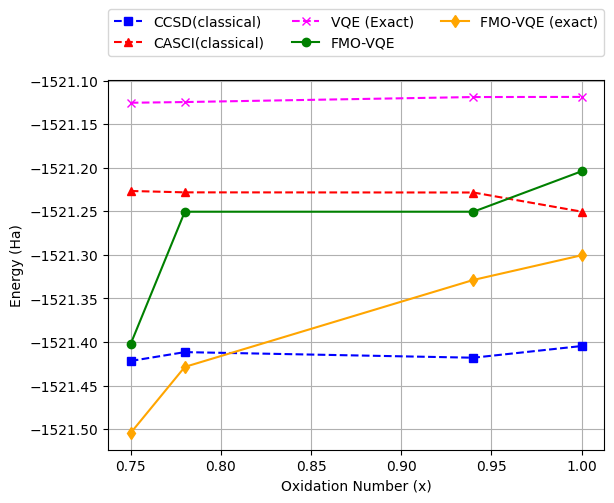
\includegraphics[width=0.8\textwidth]{fig/result2.png}
\caption{빨간색의 $"\blacktriangle"$ 마크로 표시된 점선은 CASCI를 통해 계산된 에너지를 나타낸다. 여기서 CASCI 계산의 경우 Computational Cost와 Accuracy를 균형 있게 고려하기 위해, HOMO 근방의 8개 점유 오비탈과 LUMO 근방의 4개 비점유 오비탈을 활성공간으로 선택하였다. 
파란색의 $"\blacksquare"$ 마크로 표시된 점선은 CCSD를 통해 계산된 에너지를 나타낸다. 
마젠타색의 $"\mathsf{X} "$ 마크로 표시된 점선은 FMO-VQE의 계산에서와 같은 16개의 큐비트로 계산한 VQE 알고리즘에 대응되는 결과를 나타낸다.
초록색의 $"\bullet  "$ 마크로 표시된 실선은 본 연구에서 제시하는 FMO-VQE 방식을 적용하여 얻은 결과이다. 
그리고 주황색 $"\blacklozenge "$ 로 표시된 실선은 본 연구에서 제시한 FMO-VQE 방식의 헤밀토니안을 Exact하게 풀어낸 결과이다.}\label{Fig.5}
\end{figure}

본 연구에서는 FMO-VQE 방식을 통해 제한된 큐비트 수 하에서도 보다 큰 분자 시스템의 바닥상태 에너지를 근사적으로 계산할 수 있는지를 검증하고자 하였다. 

제한된 큐비트 수에서 전통적인 VQE의 성능을 평가하기 위하여, FMO-VQE에서 사용한 것과 동일한 큐비트 수를 적용하여 VQE로부터 얻을 수 있는 최적의 결과를 산출하였다. 이를 위해 14 큐비트에 대응되도록 Hamiltonian을 구성하고, 해당 Hamiltonian을 고전적으로 대각화하여 정확한 값을 구하였다. 이 값은 VQE 알고리즘 내에서 모든 연산이 오차 없이 수행되고, 최적화 과정이 완전히 수렴한 경우에 도달할 수 있는 기준(reference) 값을 의미한다. 해당 결과는 Figure 1에서 자홍색(Magenta)으로 표시하였다. 이 전통적인 VQE 결과는 고전적 시뮬레이터(CCSD 및 FCI) 결과보다 상대적으로 높은 에너지를 나타내었으며, 이는 큐비트 수가 제한될 경우 VQE에서 생기는 최적화문제, 양자회로에 의한 오차등을 극복하더라도 전통적인 VQE 방식으로는 고전적인 계산보다 높은 정확도를 확보하기 어려움을 의미한다. 반면 FMO-VQE 방식으로 계산한 바닥상태 에너지는 CASCI 시뮬레이션 결과와 유사한 수준을 보인다. 

주황색 곡선은 본연구에서 사용한 FMO scheme을 사용하며 각 fragment의 Hamiltonian을 고전적으로 완전히 대각화하여 얻은 바닥상태 에너지를 나타낸다. 이는 이번실험에서 가정한 FMO 환경에서 VQE 계산을 통해 얻을 수 있는 가장 이상적인 결과이며 FMO-VQE 알고리즘의 기준값에 해당한다. FMO Method 를 사용한 두 결과와 FMO를 사용하지 않은 계산방법들(CCSD,UCCSD,VQE)과 비교했을 때 산화 상태에 따른 에너지 차이가 크다. 따라서 이 오차는 FMO Method 에 의한 오차라고 판단 할 수있고, 이는 본연구에서 사용한 FMO 방식에서 어떠한 상호작용이 덜 고려되었거나 더 고려되었음을 짐작할 수 있다. 그리고 이러한 오차의 이유는 fragment 간 상호작용을 나타내는 퍼텐셜 항을 생략한 데 기인하는 것으로 판단할 수 있다. 한편, FMO-VQE 결과와 주황색 기준값 사이에도 차이가 존재하는데, 이는 VQE의 최적화 과정에서 발생한 수렴 문제 또는 Barren Plateau와 같은 현상에 기인할 수 있다. 해당 오차는 최적화 전략이나 Ansatz의 개선을 통해 완화 가능할 것으로 예상된다.

이렇듯 FMO-VQE 방식은 보완할 점이 남아 있지만, 그럼에도 주목해야 하는 이유는 이 알고리즘이 가진 잠재력에 있다. 실제 계산에서는 시스템 크기에 따른 계산량 증가로 인해 완전한 FCI 계산이 사실상 불가능하며, 이에 따라 CCSD, CASCI 등 적절한 근사 기법이 연구되어 왔다. 이러한 접근들의 공통 목표는 FCI에 근접한 정확도를 유지하면서 계산 비용을 낮추는 것이다. 이 맥락에서 시스템을 조각(fragment)으로 분할해 계산하는 Fragment Molecular Orbital(FMO) 방식이 제안되었으나, 고전적 접근만으로는 계산 효율 면에서 기대에 미치지 못한다는 의견이 제시되고있다[ref. 필요함].
반면 양자적 접근에서 FMO 방식은 필요한 큐비트 수를 줄일 수 있어 NISQ 환경에서 큰 잠재력을 보인다. 
[Lim et al.]에서 제안되어 본 연구에 적용된 FMO-VQE는 전체 시스템을 작은 fragment로 분할하고 각 fragment에 VQE를 적용함으로써,
정밀도측면으로는 Fig 6. 에서 볼 수 있듯이 CASCI, CCSD 등의 기존의 계산방식과 비교하여 경쟁력 있는 결과를 얻을 수 있었으며, 계산 Cost 측면에서는 
전체 에너지 계산에 요구되는 큐비트 수를 효과적으로 감소시켰다. 특히 시스템 규모가 커질수록 필요 큐비트가 sublinear하게 증가하는 특성을 보여, NISQ 장치의 한계를 완화할 가능성을 제시한다.

물론 본 연구의 FMO-VQE 구현은 외부 전기장 항을 통한 fragment 간 상호작용의 정밀 반영, VQE 최적화 수렴 안정성 확보 등 여러 측면에서 추가 개선이 필요하다. 그럼에도 기존 VQE만으로는 접근이 어려운 시스템에 대해 근사적 에너지 계산을 수행함으로써, 복잡한 분자로의 확장 가능성과 FMO-VQE 알고리즘의 일관된 규모 확장성을 확인하였다. 비록 아직 완전하지는 않지만, 고전적으로는 사실상 불가능한 규모에서도 FMO-VQE를 통해 유효한 에너지 추정이 가능하다는 점은 향후 응용 가능성을 뒷받침한다.

% 이렇듯 FMO-VQE 방식은 보완할 점이 아직 많지만, 그럼에도 FMO-VQE 방식을 주목해야 하는 이유는, 이 방식이 가진 잠재력 때문이다. 
% 실제 계산에서는 시스템의 크기에 따라 계산량 증가로 인해 완전한 FCI 계산은 사실상 불가능하며, 적절한 근사 하에서 계산을 수행하는 방법인 CCSD, CASCI등의 방법이 연구되고있다. 
% 이러한 방식들의 주된 목적은 FCI 에 근접한 정밀도를 유지하면서 계산 Cost를 줄이는것이 주된연구분야이다. 


% 복잡한 분자 시스템의 바닥상태 에너지를 정확히 계산하는 것은 배터리 소재 설계나 신약 개발 등 다양한 분야에서 필수적인 과제가 되고 있다. 
% 그러나 시스템의 크기가 커질수록 전통적인 방법, 특히 Full Configuration Interaction(FCI)과 같은 정확한 계산 방식은 계산 자원의 급격한 증가로 인해 사실상 적용이 불가능하다.
% 이러한 맥락에서, 시스템을 조각(fragment)으로 나누어 계산하는 Fragment Molecular Orbital(FMO) 방식이 제안되어 왔으나, 고전적인 접근에서는 계산 효율성 측면에서 기대에 미치지 못한다는 의견이 제시되고있다[ref. 필요함]. 
% 하지만 양자적 접근에서 FMO 방식은 계산에 필요한 큐비트 수를 줄일 수 있으며, 이는 현재의 NISQ 환경에서 큰 잠재력을 갖는다. [Lim et al.]에서 제안되어 본 연구에 적용된 FMO-VQE 방식은 전체 시스템을 작은 fragment로 분할하고 각 fragment에 VQE를 적용함으로써 전체 에너지 계산에 요구되는 큐비트 수를 효과적으로 감소시킨다. 특히 시스템 규모가 커질수록 필요한 큐비트 수가 sublinear하게 증가하는 특성을 보여, NISQ 장치의 한계를 극복할 수 있는 가능성을 제시한다.
% 물론 본 연구에서 사용한 FMO-VQE 방식은 외부 전기장 항의 도입을 통한 fragment 간 상호작용의 정밀한 반영, VQE 최적화 과정에서의 수렴 안정성 확보 등 아직 여러 측면에서 보완이 필요하다. 그럼에도 불구하고, 본 연구는 기존 VQE 방식만으로는 사실상 접근이 어려운 시스템에 대해 근사적인 에너지 계산을 시도하였으며, 그 결과를 통해 점점 복잡한 분자를 다뤄야하는 상황에서 FMO-VQE 알고리즘이 갖는 잠재력을 확인할 수 있었다. FMO-VQE 알고리즘은 아직 완전하지는 않지만 시스템 크기 증가에 Consistent한 특징을 가지므로, 고전적으로는 계산 불가능한 상황에서 FMO-VQE 방식으로는 유효한 에너지를 계산해 낼 수 있음을 기대할 수 있다. 


% 실제 계산에서는 시스템의 크기에 따라 계산량 증가로 인해 완전한 FCI 계산은 사실상 불가능하며, 적절한 근사 하에서 계산을 수행하게 된다. 
% %이번계산에서도 FCI 로는 계산을 수행 할 수 없어 적절한 Active space를 정의하여 CASCI 방식으로 고전값을 계산하였다. 
% %따라서 지금의 양자화학 계산에서 중요한 연구는 더 좋은 근사방식을 찾는것이다. 
% 따라서, 지금의 더 복잡한 분자에 대해 양자화학 계산을 수행하기 위해서는 FMO-VQE 방식이 CASCI 나 CCSD 등의 여러 계산방법과 비교하였을때 얼마나 경쟁력있는지를 판단하는것이 중요하며, Figure 1 의 결과는 FMO-VQE 방식이 경쟁력 있는 대안이 될 수 있음을 시사한다. 
% 특히, 아직까지는 FMO-VQE 방식이 정밀도 측면에서 개선의 여지가 있음에도 불구하고, 큐비트 수가 제한된 상황에서도 비교적 정확한 에너지를 근사할 수 있다는 점은 주목할 만하다.

\section{Conclusions}
본 연구에서는 양자 알고리즘인 FMO-VQE 방식을 적용하여, \(\mathrm{LiCoO_2}\)  분자의 바닥상태 에너지를 고전적인 시뮬레이터와 비교하였다. 본 연구에서는 아직 초기단계의 시도로써, 작은 basis sets을 사용하였고, FMO 방식에서 Fragment의 외부 전기장 항을 무시하여, 화학적인 해석에 있어서 유의미한 결과는 얻지는 못하였지만, 
동일하게 제한된 큐비트를 사용한 VQE 알고리즘의 Optimal 한 결과와 고전적 양자화학 계산 알고리즘 (CCSD, CASCI 등)와의 비교를 통해 통해 FMO-VQE 방식의 정밀도와 신뢰성을 평가할 수 있었다.
기존의 계산량 문제에 대한 해결책으로 VQE 알고리즘이 제안되었으나, 현재의 NISQ(Noisy Intermediate-Scale Quantum) 시대에는 제한된 양자 하드웨어 성능으로 인해 그 실용성에 대한 기대가 다소 약화된 상황이다. 그러나 본 연구에서 제안하는 FMO-VQE 방식은, 이러한 하드웨어 제약 하에서도 양자 하드웨어의 이점을 실제 계산에 활용할 수 있는 가능성을 제시한다.
즉, 더욱 복잡한 분자를 다룰 때 기존의 알고리즘으로는 유효한 에너지를 계산할 수 없는 경우에도, FMO-VQE 방식에서는 양자 하드웨어의 이점을 이용하여 동일한 수준의 근사 하에서 보다 정확한 에너지를 계산할 수 있을 것으로 기대된다. 이러한 결과는 향후 신약 합성 및 신소재 개발과 같은 복잡한 분자 시스템이 요구되는 분야에서, 계산량의 제약으로 인해 발생할 수 있는 문제에 대한 해결책으로 FMO-VQE가 활용될 수 있음을 시사한다. 
본 연구는 아직 초기 단계의 시도로써, 고전적으로는 큰 효과가 없는 FMO 방식이 양자적으로 VQE와 함께 적용할때는 계산에 필요한 큐비트를 줄이면서 고전적인 계산방법과 비슷한 정밀도를 얻을수 있음을 기대할 수 있는 결과를 얻었다. 즉, 이번 연구는 FMO-VQE 방식이 복잡한 분자의 양자화학 계산에 새로운 계산 패러다임으로 작용할 수 있음을 제시하며, 향후 FMO 방식의 개선을 통해 다양한 양자 시스템 및 화학적 조건에 대한 확장 가능성을 보여준다.

% \bibliographystyle{plain}
\bibliography{FMOVQE_Ref}

\end{document}

